\chapter{Fit structure and results}
\label{ch:fit}
%\epigraph{\itshape``Tiny details imperceptible to us decide everything!"}{--- \textup{Winfried Georg Sebald, Vertigo}}
\epigraph{\itshape``What could I say to you that would be of value, except that perhaps you seek too much, that as a result of your seeking you cannot find. "}{--- \textup{Hermann Hesse}}

\section{Introduction}
\hspace{10pt} Before proceeding with the discussion of the final result representing this study, an overview of all analysis inputs needs to be made in order to summarise constituents entering the final measurement. The following sections are going introduce the fit strategy, presented in terms of the signal extraction approach, coupled with a general introduction to the statistical apparatus. Building on that general topic, the next item of discussion is going to be the formation of the likelihood function for the searches of the invisible state. It will be shown how it summarises the information from dedicated control regions as well as from the signal region.

\hspace{10pt} Following the summary of contributions from each region, the focus is going to be placed on the overview of theoretical and experimental uncertainties. This discussion will split into two distinct parts. The first one will be focusing on theoretical uncertainties and will encapsulate details regarding their rise from the NLO corrections on V+jets simulation samples. On the other hand, the second part will be comprised from a discussion of experimental uncertainties covering various sources.

%\hspace{10pt} An important topic covering the validation of transfer factors connecting the CR to SR contribution of V+jets backgrounds is going to be introduced alongside a summary of results following QCD estimation techniques (introduced in Chapter~\ref{ch:control_regions}). This will help with rounding up the story of main SM backgrounds.

\hspace{10pt} Lastly, the third act of this chapter serves as a summary of results arising from measurements defined by previously introduced strategy. The related sections are going to be dedicated to measurements through the usage of data collected by the CMS experiment during the 2017 and 2018 eras of data taking. A discussion of benefits rising due to the inclusion of a new analysis category, formed around the VBF triggers, is also presented. Final result from the VBF H$\rightarrow$inv analysis from the perspective of the full Run 2 era is obtained through a combination with, previously published, study detailing the analysis of 2016 data~\cite{paper:HIG_17_023}.
\section{The CLs approach}

\hspace{10pt} The characteristics of the VBF topology are manifested through the existence of two jets. Through an optimisation technique it was shown that the largest signal versus background shape separation is gained when deploying the dijet invariant mass as the main analysis tool\footnote{More details about the jet properties from the perspective of the VBF production mode are given in Chapter~\ref{ch:an_strategy}.}~\cite{paper:HIG_17_023,Riccardo}. For a measurement of the aforemnetioned property, the resulting data can be represented with a binned histogram (with $d_i$ denoting a certain mass bin). Due to the nature of collider experiments, the use of Poisson statistics is applicable to studies of this kind. This allows for the introduction of the binned likelihood function as:

\begin{equation}
   \small{\mathcal{L}(\mu, \boldsymbol{\theta}) = \prod_i \frac{(\mu S_i(\boldsymbol{\theta})+B_i(\boldsymbol{\theta}))^{d_i}e^{-(\mu S_i(\boldsymbol{\theta})+B_i(\boldsymbol{\theta}))}}{d_i!} = \prod_i \text{Pois}(d_i|(\mu S_i(\boldsymbol{\theta})+B_i(\boldsymbol{\theta})),}
    \label{eq:likelihood_def}
\end{equation}

where the terms comprising the product can be interpreted as the probabilities that $d_i$ occurences of the dijet mass confined to the bin range of $i$ has been observed given the expected valued of events being $\mu S_i(\boldsymbol{\theta})+B_i(\boldsymbol{\theta})$~\cite{paper:stat_overview,paper:cls_intro}. The bin values associated with the signal ($S_i(\boldsymbol{\theta})$) and background ($B_i(\boldsymbol{\theta})$ processes are obtained from the simulation of SM processes and the dependency on a set of nuisance parameters $\boldsymbol{\theta}$. Lastly, the $\mu$ is a free parameter in the fit and in this scenario it represents the desired branching ratio. The test statistic can now be formed as: $q_\mu = -2ln\frac{\mathcal{L}(\mu, \boldsymbol{\theta(\mu)})}{\mathcal{L}(\mu_m, \boldsymbol{\theta_m})}$, where $\mu_m$ and $\theta_m$ represent the values of the parameters yielding the largest value of the Likelihood funcion, and $\theta(\mu)$ denotes the value of a parameter $\theta$ which maximises the Likelihood function for a given choice of $\mu$. 

\hspace{10pt} When approaching the task of setting a limit on the probability of the Higgs boson decaying invisibly, one must propose a way of thinking opposite to the case when there is a hunt for a discovery. In these scenarios, the null hypothesis ($H_0$) is represented by the signal~$+$~background scenario which is compared to the alternative ($H_1$) denoted as background only scenario (as introduced in Ref.~\cite{paper:stat_overview}). For the purposes of the VBF H$\rightarrow$inv search that would introduce the options of including the SM Higgs by fixing the values of Br(H$\rightarrow$inv) to be 1 or 0 respectively. Following from the previous definitions, the final comparison can be made by following the CLs criterion~\cite{paper:stat_overview,paper:cls_intro}, through which the value of the 95\% CL upper limit on Br(H$\rightarrow$~inv) is obtained.

\hspace{10pt} This simplified method of having only one region represented with $\mu S_i+B_i$ is used to illustrate the entire process without the pressure of multiple additional background enriched regions. The details of their inclusion into the signal extraction procedure are the focal point of the following section.
\section{Signal extraction strategy}
\hspace{10pt} The information gathered from four lepton control regions (described in Chapter~\ref{ch:control_regions}) and the signal region (with both analysis categories being defined in Chapter~\ref{ch:an_strategy}) is used when forming of the, $m_{jj}$ binned, likelihood function. It is formed in such a way that it allows the fit to simultaneously access all available information, with the end result of having a final estimate of the contribution originating from Z$\rightarrow \nu\nu$+jets and W$\rightarrow l\nu$+jets irreducible backgrounds. The formation of the likelihood function can be split in the following way:

\begin{equation}
   \small{ \mathcal{L}(\boldsymbol{\mu}^{Z\rightarrow \nu\nu}, \boldsymbol{\mu}, \boldsymbol{\theta}) =  \mathcal{L}_{SR}\times \prod_{j = \mu, e} \mathcal{L}_{CR,Z}^i \times \prod_{k = \mu, e} \mathcal{L}_{CR,W}^j\times\prod_{l}\text{P}(\theta_l) ,}
    \label{eq:likelihood_total}
\end{equation}

where $\boldsymbol{\mu}^{Z\rightarrow \nu\nu} = (\mu_i^{Z\rightarrow \nu\nu})$ summarises the binned contribution of QCD $Z\rightarrow \nu\nu$ SM background processes and $\boldsymbol{\mu}$ represents the signal strength parameter. Both of these are free parameters withing the fit. Additionally, $\boldsymbol{\theta} = (\theta_l)$ symbol is used to summarise systematic uncertainties included in the likelihood in the form of constrained nuisance parameters ($P(\theta_l)$ terms\footnote{Represented with Gaussian or log-normal functions.}).

\hspace{10pt} Starting with the first member of the likelihood function, the likelihood function representing the information given by the SR, akin to the one previously introduced with Equation~\ref{eq:likelihood_def}, can be written down as:

\begin{equation}
 \small{\mathcal{L}_{SR} =  \prod_{i} \mathrm{Pois}\left(d_{i} | B_{i}(\boldsymbol{\theta}) + (1+f_{i}(\boldsymbol{\theta})_{\mathrm{QCD}}) \mu_{i}^{Z\rightarrow \nu\nu} + R^{\frac{EWK}{QCD}}_{i} (1+f_{i}(\boldsymbol{\theta})_{\mathrm{EWK}}) \mu_{i}^{Z\rightarrow \nu\nu}+ \boldsymbol{\mu} S_{i}(\boldsymbol{\theta})\right ),}
\end{equation}

where $d_i$ represents the number of events observed in data for a given $m_{jj}$ bin $i$, and $B_i$ and $S_i$ define the total background and nominal signal yields within the same bin range. With the $\mu_i^{Z\rightarrow \nu\nu}$ being a free parameters, a parameter $R^{\frac{EWK}{QCD}}_{i}$ is introduced in order to connect the SR contribution from EWK and QCD producitions of $Z\rightarrow \nu\nu$+jets processes (estimated from simulation\footnote{Does not posses any additional uncertainty.}). Lastly, a connection with the W$\rightarrow l\nu$+jets processes is introduced through the addition of $f_i(\theta)_{QCD} = \frac{SR^{Z\rightarrow \nu\nu}_{QCD}}{SR^{W\rightarrow l\nu}_{QCD}}$, which represents a ratio of simulated contributions of these two backgrounds in the SR. It serves as a connection between these two sources of backgrounds (equivalent definition follows for the EWK production).

\hspace{10pt} The contribution from each of the dilepton CRs, using the dielectron region as an example, can be summarised as:

\begin{equation}
\small
  \small{\mathcal{L}_{CR,Z}^{e} = \prod_{i} \mathrm{Pois} \left(d^{Z}_{i}|B^{Z}_{i}(\boldsymbol{\theta}) +\frac{\mu_i^{Z\rightarrow \nu\nu}}{R^{Z}_{i} (\boldsymbol{\theta})_{\mathrm{QCD}}} + R^{\frac{EWK}{QCD}}_{i}\cdot\frac{\mu_i^{Z\rightarrow \nu\nu} }{R^{Z}_{i} (\boldsymbol{\theta})_{\mathrm{EWK}}} \right).}
    \label{eq:likelihood_dilepton}
\end{equation}

where $d_i^Z$ represents the number of events observed in data for a given $m_{jj}$ bin $i$, and the ratios $R_i^Z(\boldsymbol{\theta})_{QCD}$ and $R_i^Z(\boldsymbol{\theta})_{EWK}$ represent transfer factors which connect the overall CR yields of QCD (EWK) Z$\rightarrow ll$+jets processes with their QCD (EWK) Z$\rightarrow \nu\nu$+jets counterparts in the SR (again within the given $m_{jj}$ bin range). The single lepton constituent follows a similar idea and can be defined as \footnote{Again using electron region as the example}:

\begin{equation}
\small{
    \mathcal{L}_{CR,W}^{e} = \prod_{i} \mathrm{Pois} \left(d^{W}_{i}|B^{W}_{i}(\boldsymbol{\theta}) + f_i(\boldsymbol{\theta})_{QCD} \cdot \frac{\mu_i^{Z\rightarrow \nu\nu}}{R^{W}_{i} (\boldsymbol{\theta})_{\mathrm{QCD}}} + R^{\frac{EWK}{QCD}}_{i} \cdot f_i(\boldsymbol{\theta})_{EWK} \cdot \frac{\mu_i^{Z\rightarrow \nu\nu} }{R^{W}_{i} (\boldsymbol{\theta})_{\mathrm{EWK}}} \right),}
\end{equation}

where the definitions of transfer factors follow their dilepton counterparts. These, followed with their muon variants, construct the likelihood function introduced in Equation~\ref{eq:likelihood_total}. For the MTR category there is one more constituent added to this definition, a product of Poissonian terms focusing on the photon region. Following a similar blueprint (and motivation), the photon CR is added in order to aid with the constrain of the $Z\rightarrow \nu\nu$+jets SM background. Its topology, for large values of photon transverse momenta, follows a similar trend as $Z\rightarrow \nu\nu$+jets. The formation of this region requires exactly one loose photon in the event, having no additional photons or leptons, with the dijet topology requirements being placed on top of it. The likelihood contribution of the photon region is equivalent to the one definied for dilepton regions in Equation~\ref{eq:likelihood_dilepton}\footnote{With the redefintion of the transfer factors in order to include the information coming from the photon region.}.
%This relation is estimated using simulated events and can be expressed as\footnote{ Continuing using the dielectron region as an example.}:

%\begin{equation}
%R_{i}^Z(\boldsymbol{\theta})_{QCD} = \frac{SR_{i}^{Z\rightarrow\nu\nu}}{CR_{i}^{Z\rightarrow ee}},
%\end{equation}

%where $X_{i,MC}^{V}$ represents number of events of a given SM process in the dedicated region $X$\footnote{Where $X =$~SR or CR (in this case the dielectron CR).}, expressed in $m_{jj}$ bins.

%\begingroup
%\small
%\begin{align}
%\mathcal{L}(\boldsymbol{\mu}^{Z\rightarrow \nu\nu}, \boldsymbol{\mu}, \boldsymbol{\theta}) = &
%\prod_{i} \mathrm{Pois}\left(d_{i} | B_{i}(\boldsymbol{\theta}) + (1+f_{i}(\boldsymbol{\theta})_{\mathrm{QCD}}) \muz_{i} + R^{EW/QCD}_{i} %(1+f_{i}(\boldsymbol{\theta})_{\mathrm{EW}}) \muz_{i}+ \boldsymbol{\mu} S_{i}(\boldsymbol{\theta})\right ) \times \nonumber\\
%&\prod_{i} \mathrm{Pois} \left(d^{Z}_{i}|B^{Z}_{i}(\boldsymbol{\theta}) +\frac{\muz_{i} }{R^{Z}_{i} (\boldsymbol{\theta})_{\mathrm{QCD}}} + \frac{\muz_{i} }{R^{Z}_{i} (\boldsymbol{\theta})_{\mathrm{EW}}} \right) \times \nonumber\\
%& \prod_{i} \mathrm{Pois}\left(d^{W}_{i}|B^{W}_{i}(\boldsymbol{\theta}) +\frac{f_{i}(\boldsymbol{\theta})_{\mathrm{QCD}}\,\muz_{i}}{R^{W}_{i}(\boldsymbol{\theta})_{\mathrm{QCD}}}+\frac{f_{i}(\boldsymbol{\theta})_{\mathrm{EW}}\,\muz_{i} }{R^{W}_{i} (\boldsymbol{\theta})_{\mathrm{EW}}} \right) \times \nonumber\\
%& \prod_{i} \mathrm{Pois}\left(d^{\gamma}_{i}|B^{\gamma}_{i}(\boldsymbol{\theta}) +\frac{\muz_{i}}{R^{\gamma}_{i}(\boldsymbol{\theta})_{\mathrm{QCD}}}+\frac{\muz_{i} }{R^{\gamma}_{i} (\boldsymbol{\theta})_{\mathrm{EW}}} \right) \nonumber,\\
%\end{align}
%\endgroup

%where $\mu^{Z\rigtharrow\nu\nu}_i$ denotes the binned contribution from Z$\rightarrow\nu\nu$+jets processes in the SR, the $\mu$ parameter represents the signal strength and $\theta$ is used to summarise systematic uncertainties (whose treatment is going to be the focus of Section~[R]). In order to efficiently present its contents, each line of the previously defined likelihood function is separated by its respective information group with the Z or W indices marking the contribution origination from respective lepton regions whereas the EWK/QCD notation is used to separate the information based on the production mode.

%\hspace{10pt} The general idea behind the fit is that the binned contribution from Z$\rightarrow \nu\nu$+jets backgrounds is set to be a free parameter alongside the signal strength. The separation by production mode states that the final yields of V+jets backgrounds are going to be estimate per its EWK/QCD modes. The fit itself is constrained with the connection between the main Z$\rightarrow\nu\nu$+jets backgrounds in the form of parameters $R_i^{EWK/QCD}$. This parameter represents the ratio of contributions coming from EWK and QCD components of the Z$\rightarrow\nu\nu$ process and doesn't have any other associated uncertainties. The $f_i(\theta)$ functions are used to express the ratio between ratios (transfer factors) between the Z$\rightarrow \nu\nu$+jets and W$\rightarrow l\nu$ processes through their respective contributions in the SR (representing a constrain between these sources of background). Uncertainties which associated with transfer factors enter the likelihood functions as additive perturbations (being modelled as Gaussians). The likelihood function includes the contribution from background sources ($B_i$) and the nominal signal prediction ($S$) in the SR.


%\hspace{10pt} Starting with the dilepton regions and the relation of Z$\rightarrow ll$+jets yields to the all neutrino decay of the Z boson in the SR. These ratios take into account for differences originating from multiple sources: values of branching ratios for different final states, lepton selection and veto efficiencies as well as the difference in trigger performance for the dielectron case. These transfer factors are validated through Figure~[R], where a ratio between the $Z\rightarrow\mu\mu$ and $ee$ is compared between the data (subtracted from minor background contributions) and Z+jets simulation (inclusive of both production modes). A similar approach is taken when approaching the W$\rightarrow l\nu$+jets backgrounds. The corresponding validation plots are shown in Figure~[R] for both muon and electron regions.


%\begin{figure}[htbp]
%  \centering
%    \includegraphics[width=0.49 \textwidth]{example-image-a}
%    \includegraphics[width=0.49\textwidth]{example-image-a}

%  \caption{Diagram of the event categorisation used for the combined H$\rightarrow$inv study~\cite{note:AN_18_299,note:AN_19_257}}
%  \label{fig:chip}
%\end{figure}

%\begin{figure}[htbp]
%  \centering
%    \includegraphics[width=0.49 \textwidth]{example-image-a}
%    \includegraphics[width=0.49\textwidth]{example-image-a}

%  \caption{Diagram of the event categorisation used for the combined H$\rightarrow$inv study~\cite{note:AN_18_299,note:AN_19_257}}
%  \label{fig:chip}
%\end{figure}



\section{Treatment of uncertainties}
\hspace{10pt} The systematic uncertainties play a significant role in these measurements and can be either a result of higher order theory corrections applied on the LO simulation samples (as explained in Chapter~\ref{ch:objects}) or they can be associated to one of multiple experimental sources. The following sections detail each of these groups.

\subsection{Theoretical uncertainties}
\hspace{10pt} Simulated samples of the main signal processes, the VBF and ggH productions, have associated uncertainties originating from factorization, renormalization and parton density function (PDF) variations [R]. The ggH production has additional sources of uncertainty coming from limited information about the ggH+X\footnote{Where the X represents scenarios with two or more additional jets.} cross sections and the uncertainty related to the prediction of the ggH cross section for large values of $p_T^{H}$\footnote{$p_T^{H}>$~250~GeV.}. This totals to an additional 40~\% uncertainty. Lastly, due to the choice of the PDF set, uncertainty associated to the signal acceptance is treated per process.

\hspace{10pt} Theoretical uncertainties have an effect on the transfer factors $f(\boldsymbol{\theta})$\footnote{These rest of the Z and W transfer factors they are expected to cancel out due to similar jet topological properties between the SR and respective CRs}. The core of these of uncertainties is represented with the effects connected to the EWK and QCD higher order corrections coupled with the uncertainty associated with the PDF modeling. The first item taken into consideration arises due to the variations revolving the choice of the central renormalization and factorization scale. These variations involve changing both scales by increasing or decreasing them by a factor of two with respect to its nominal value. This is reflected in the final weights being used in the analysis. These uncertainties are assumed to be partially correlated between the W and Z samples. Taking a more conservative approach when estimating their effect on the $f(\boldsymbol{\theta})$ ratios, only the W variation (as the larger contribution) is considered. These final uncertainties are used for both the EWK and QCD variations of the transfer factor $f(\boldsymbol{\theta})$.

Figure~[R] shows the uncertainties on the $f(\boldsymbol{\theta})$ transfer factor for the MTR category for the 2017 data (with the rest of the categories being represented with Figures~[A]-[A]).
%As these corrections are being applied as a two dimensional weight map in generator level boson $p_T$ and $m_{jj}$ (as discussed in Chapter~\ref{ch:objects}), the final uncertainties are derived through the differences between the NLO cross sections (expressed in boson $p_T$ and $m_{jj}$) corresponding to the variated and nominal scenario. Finally, the uncertainty originating from the PDF modelling is estimated through a procedure recommended by the PDF4LHC working group~[R] and combined with other sources through a squared sum. 
 
\subsection{Experimental uncertainties}
\hspace{10pt} The experimental uncertainties are related to the effects of the performance of the detector and the object reconstruction. Sources comprising this group include pileup re-weighting, trigger performance, jet energy corrections (both the scale and resolution) and object reconstruction and isolation criteria (expressed through the usage of selection/veto weights as explained in Chapter~\ref{ch:objects}). Table~\ref{tab:systematics} summarises the experimental uncertainties on V+jets transfer factors, while Table~\ref{tab:systematics_minor} summarises the respective uncertainties on smaller backgrounds.


\begin{table}[htbp]

\small
    \begin{center}
       \begin{tabular}{llc}
       \hline
       \hline
       Source                    & Process                                    & Uncertainty  \\
       \hline
       \hline
       Electron  trigger         & $W_{SR}/W_{e\nu}$, $Z_{\nu\nu}/Z_{ee}$       & 1\% \\
       \MET   triggers             & $W_{SR}/W_{CR}$, $Z_{\nu\nu}/Z_{CR}$, $Z/W$, signal & 2\% \\
       VBF  triggers             & signal  & 10\% \\
%       Photon  trigger           & $Z_{\nu\nu}/\gamma$                           & 1\% \\
       \hline
       Muon-ID   efficiency      & $W_{SR}/W_{\mu\nu}$, $Z_{\nu\nu}/Z_{\mu\mu}$ & 0.5\% (per leg) \\
       Muon-Iso   efficiency     & $W_{SR}/W_{\mu\nu}$, $Z_{\nu\nu}/Z_{\mu\mu}$ & 0.1\% (per leg) \\
       Electron-reco efficiency  & $W_{SR}/W_{e\nu}$, $Z_{\nu\nu}/Z_{ee}$       & 0.5\% (per leg) \\
       Electron-IDiso efficiency & $W_{SR}/W_{e\nu}$, $Z_{\nu\nu}/Z_{ee}$       & 3\% (per leg) \\
 %      Photon-IDiso efficiency   & $Z_{\nu\nu}/\gamma$       & 5\% \\
      \hline
      Electron veto from reco &  $W_{l,SR}$, $Z/W$  & 1\% (QCD), 1.5\% (EW)\\
      Electron veto from idiso &  $W_{l,SR}$, $Z/W$  & 3\% \\
      Muon veto &  $W_{l,SR}$, $Z/W$  & 0.5\% \\
      Tau veto &  $W_{l,SR}$, $Z/W$  & 1\% \\
      \hline
       \multirow{4}{*}{Jet energy scale}         & $Z/W$         & 1--2\%\\
                                & $W_{CR}/W_{SR}$               & 1.0--1.5\% \\
                               	& $Z_{CR}/Z_{\nu\nu}$   		& 1\% \\
 %                              	& $Z_{\nu\nu}/\gamma$	    	& 3\% \\\hline
       \multirow{4}{*}{Jet energy resolution}  	& $Z/W$         & 1.0--2.5\% \\ 
                                & $W_{CR}/W_{SR}$               & 1.0--1.5\% \\
                                & $Z_{CR}/Z_{SR}$				& 1\% \\
 %                               & $Z_{\nu\nu}/\gamma$	    	& 1--4\% \\
       \hline
       %pileup & all ratios & 1\% \\
      \end{tabular}
    \end{center}
    \label{tab:systematics}
        \caption{Summary of experimental uncertainties in the transfer factors between main V+jets backgrounds. Where specified in the form of a range of values, the values vary with era of data taking and between different EWK or QCD induced jets.}
\end{table}


\begin{table}[htbp]

\small
    \begin{center}
       \begin{tabular}{llc}
       \hline
       \hline
       Source                    & Process                                    & Uncertainty  \\
       \hline
       \hline
       Electron  trigger         & $W_{SR}/W_{e\nu}$, $Z_{\nu\nu}/Z_{ee}$       & 1\% \\
       \MET   triggers             & $W_{SR}/W_{CR}$, $Z_{\nu\nu}/Z_{CR}$, $Z/W$, signal & 2\% \\
       VBF  triggers             & signal  & 10\% \\
%       Photon  trigger           & $Z_{\nu\nu}/\gamma$                           & 1\% \\
       \hline
       Muon-ID   efficiency      & $W_{SR}/W_{\mu\nu}$, $Z_{\nu\nu}/Z_{\mu\mu}$ & 0.5\% (per leg) \\
       Muon-Iso   efficiency     & $W_{SR}/W_{\mu\nu}$, $Z_{\nu\nu}/Z_{\mu\mu}$ & 0.1\% (per leg) \\
       Electron-reco efficiency  & $W_{SR}/W_{e\nu}$, $Z_{\nu\nu}/Z_{ee}$       & 0.5\% (per leg) \\
       Electron-IDiso efficiency & $W_{SR}/W_{e\nu}$, $Z_{\nu\nu}/Z_{ee}$       & 3\% (per leg) \\
 %      Photon-IDiso efficiency   & $Z_{\nu\nu}/\gamma$       & 5\% \\
      \hline
      Electron veto from reco &  $W_{l,SR}$, $Z/W$  & 1\% (QCD), 1.5\% (EW)\\
      Electron veto from idiso &  $W_{l,SR}$, $Z/W$  & 3\% \\
      Muon veto &  $W_{l,SR}$, $Z/W$  & 0.5\% \\
      Tau veto &  $W_{l,SR}$, $Z/W$  & 1\% \\
      \hline
       \multirow{4}{*}{Jet energy scale}         & $Z/W$         & 1--2\%\\
                                & $W_{CR}/W_{SR}$               & 1.0--1.5\% \\
                               	& $Z_{CR}/Z_{\nu\nu}$   		& 1\% \\
 %                              	& $Z_{\nu\nu}/\gamma$	    	& 3\% \\\hline
       \multirow{4}{*}{Jet energy resolution}  	& $Z/W$         & 1.0--2.5\% \\ 
                                & $W_{CR}/W_{SR}$               & 1.0--1.5\% \\
                                & $Z_{CR}/Z_{SR}$				& 1\% \\
 %                               & $Z_{\nu\nu}/\gamma$	    	& 1--4\% \\
       \hline
       %pileup & all ratios & 1\% \\
      \end{tabular}
    \end{center}
    \label{tab:systematics}
        \caption{Summary of experimental uncertainties in the transfer factors between smaller backgrounds. Where specified in the form of a range of values (PLACEHOLDER).}
\end{table}

\section{QCD estimation}


\newpage

\section{Results}

\hspace{10pt} The signal extraction procedure introduced in previous sections is applied to all regions simultaneously. This section summarises the final results, expressed in terms of the 95~\% CL upper limit on Br(H$\rightarrow$~inv)\footnote{As no significant deviations from the SM have been observed.} for all analysis categories. In order to formulate a preliminary look at the combined Run 2 (or the "legacy") result, a combination is performed with the studies targeting the 2016 data without re-analysing the data (being explained in great detail in Refs. [R,R]). Treatment of most important nuisance parameters, such as the ones related to lepton efficiencies, have been left uncorrelated between the three years with the uncertainties assigned to the jet energy scale and resolution also following the uncorrelated path. A correlation between theory uncertainty has been established between 2017 and 2018 (although they differ between MTR and VTR categories). The addition of the photon region has been performed for the MTR category for the 2017 and 2018 eras of data taking.

\hspace{10pt} Starting with the main analysis category, Figures~[R]-[R] show postfit distributions for the main CRs and the SR. Tables~[R]-[R] present the final yields in the SR for the MTR category. No excess is present at the moment TBA discussion of the results.

\hspace{10pt} The resulting postfit distributions associated to the VTR category are shown in Figures~[R]-[R]. The corresponding yields of data and simulated SM processes are given in Tables~[R]-[R].


\section{Summary}
\hspace{10pt} The presented study covered the search for the invisible decays of the Higgs boson, where the production mode in question is VBF, The study was performed using the 101.3~$fb^{-1}$ of data collected by the CMS experiment. Exploration of additional phase space found in lower $E_{T,miss}$ range was enabled through the introduction of a new analysis category based on new trigger algorithms tailored to look for the VBF topology. No deviations from the SM have been observed. The result is interpreted as the observed (expected) 95\% CL upper limit on the branching ratio of the Higgs boson decaying invisibly and it stands at: Br(H$\rightarrow$inv) = XX (XX). A combination with previous measurements targeting the VBF topology during the Run 2 phase is presented, bringing the total integrated luminosity to 137.2~$fb^{-1}$. The observed (expected) value of the Br(H$\rightarrow$inv) for the entire Run 2 phase is found to be XX (XX)\footnote{Under the assumption of the SM production cross section.}. Figure~\ref{fig:combined_limit} summarised the results of the individual measurements and the subsequent combination of categories.

\begin{figure}[htbp]
  \centering
    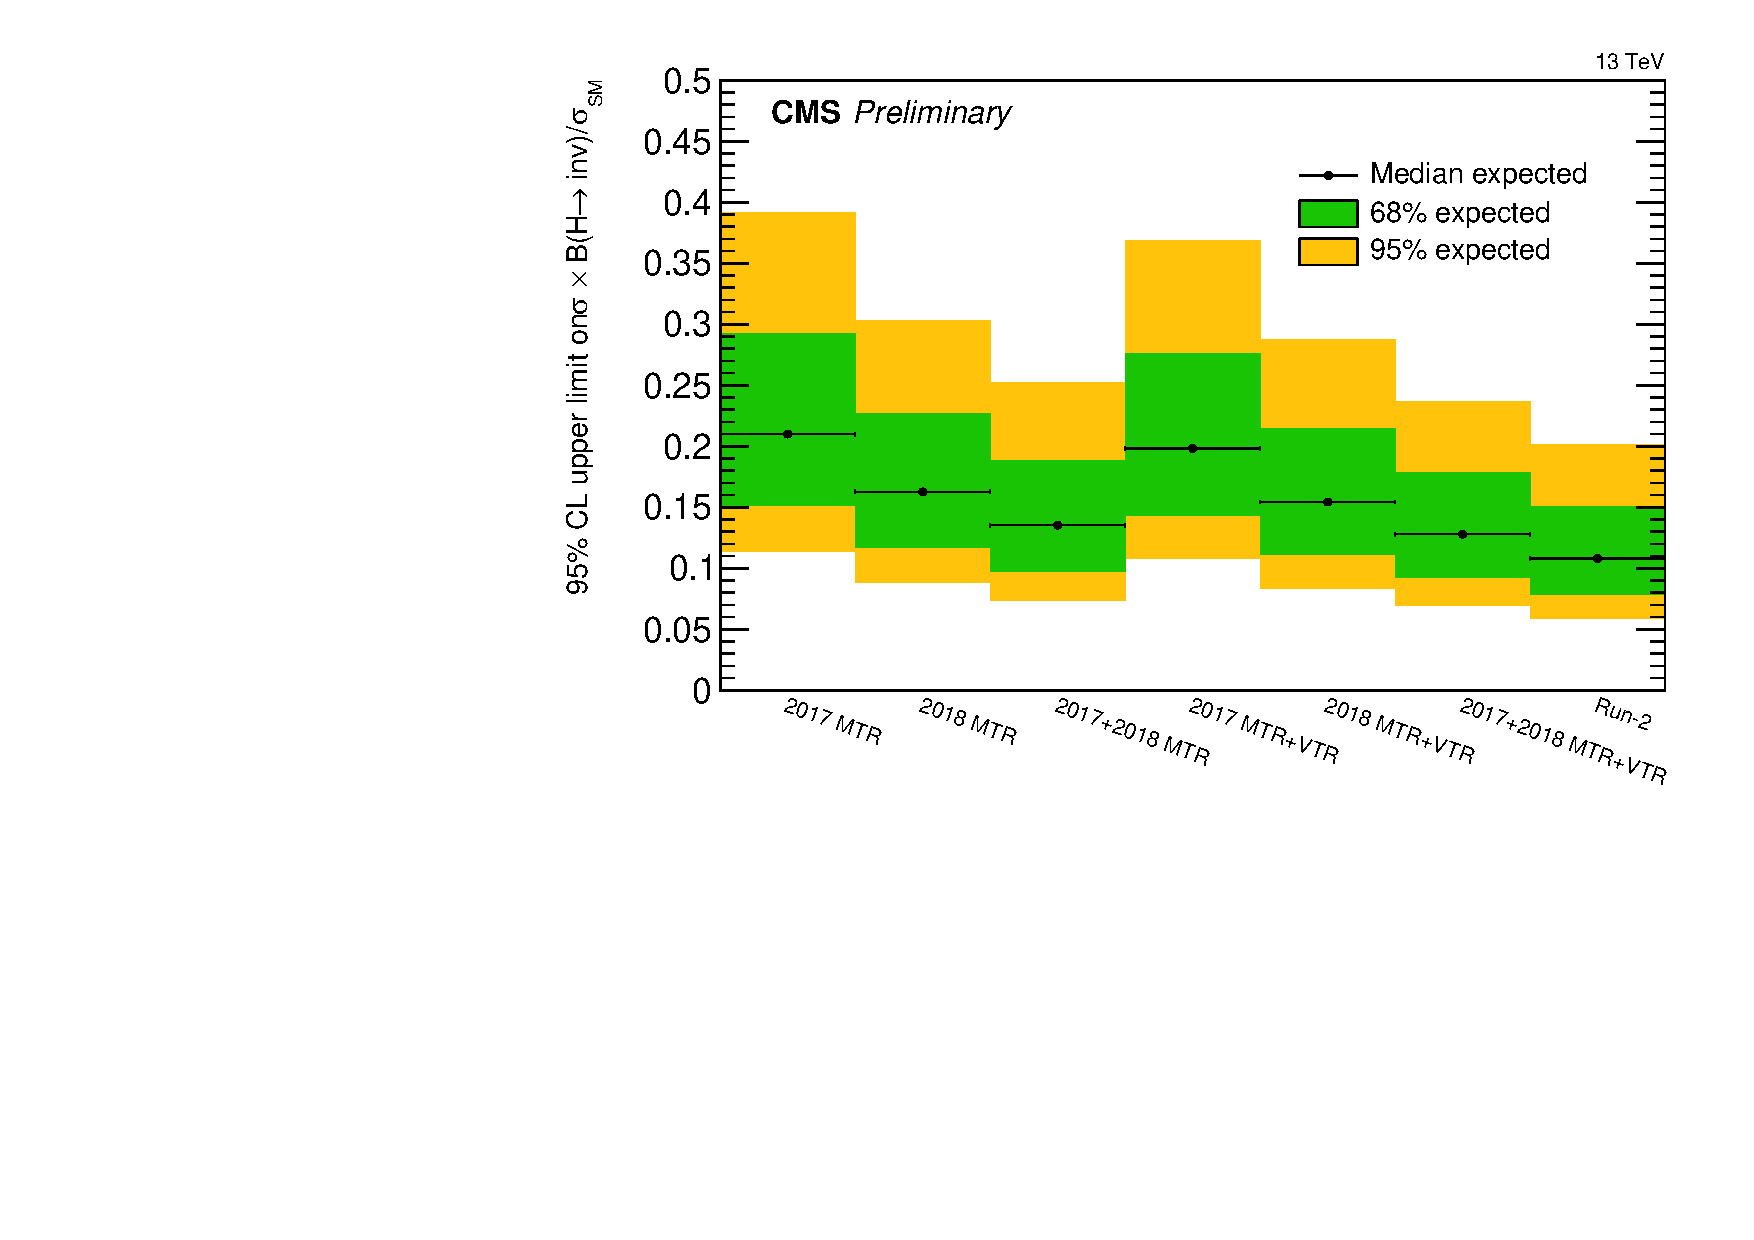
\includegraphics[width= 0.95\textwidth]{Results/limit.pdf}
  \caption{Combined limit (PLACEHOLDER).}
  \label{fig:combined_limit}
\end{figure}